\chapter{The Sagnac-Speedmeter Experiment}
\label{c:speedmeter-intro}

\section{Concept}
* Show Michelson response and noise. This should be radiation pressure dominated below the pole. Relate this to the analytical response equation I used in the controls paper for a Michelson.
* Introduce Sagnac speedmeter, showing it has better quantum noise IN ABSENCE OF ASYMMETRIES, and thus better overall sensitivity for equivalent shot noise.
* Introduce losses to show the degrading effect they have, introducing ``Michelson-like'' sensitivity. The main thing to show here is the effect on the quantum noise when there are asymmetries, like test mass asymmetry. This broadens the peak around the suspension resonance, which introduces the Michelson-like sensitivity.

\section{Implementation}

Some technical challenges in the implementation of the speedmeter are discussed in this chapter. Certain topics involve substantially more scientific endeavour and are thus presented as discrete chapters: the control of the primary degree of freedom of the speedmeter, presented in Chapter X; and a proof-of-principle experiment to demonstrate a new type of actuator, presented in Chapter Y.

\subsection{Wiring}
\note{Avoidance of ground loops, interfacing with CDS, avoiding plugging the wrong things in (why we use D-sub-9 and D-sub-15), in-vacuum wiring: why it needs careful thought, and what we did (octopus cables, etc.).}
\note{Avoidance of ground loops}
\note{Auxiliary coil driver subrack wiring design / motivation / assembly}
\note{In-vacuum cabling design, strain relief housing}
\note{Backplane board design - talk about rationale, show Eagle diagrams, etc.}
\note{Display wiring diagrams in landscape mode, full page}

\note{Generate A4 versions of wiring diagrams for inclusion here.}

\begin{figure}
  \centering
  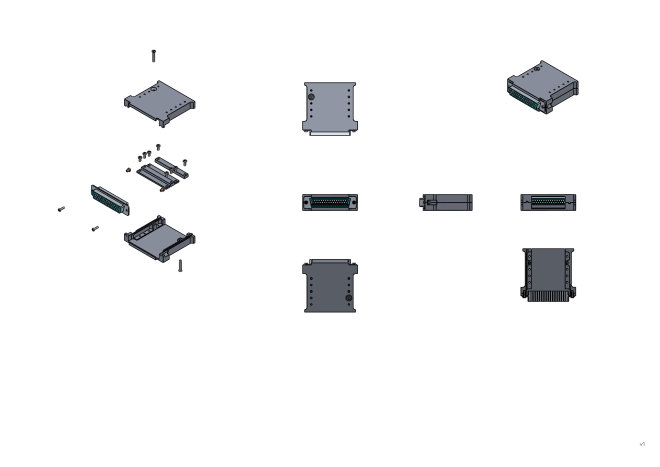
\includegraphics[width=0.75\columnwidth]{graphics/50-db50-housing.png}
  \caption{In-vacuum DB50 housing for octopus cable.}
  \label{fig:db50-housing}
\end{figure}